\documentclass[a4paper,10pt]{article} % Type de document : article scientifique
\usepackage[top=0.5cm,bottom=2.5cm,right=2.5cm,left=2.5cm]{geometry}
\usepackage[T1]{fontenc}
\usepackage[francais]{babel} % Traduction en français
\usepackage[utf8]{inputenc} % Autorise les caractères accentués
\usepackage{amsmath}
\usepackage{listings}
\usepackage{matlab-prettifier}
\usepackage{graphicx}
%\pagecolor[rgb]{0.074,0.066,0.070}
%\color{white}
\title{\textbf{Forme canonique d'une fonction polynôme de degré 2}} % Titre du document
\author{Josselin Fatah-Roux\\\\
	Titulaire d'un Master Physique Sciences de l'Ingénieur\\
	https://ovnie.com/cv/reports/index.html\\
	\texttt{vufic@outlook.com}} % Auteur
\date{\today} % Date de création
\begin{document} % Début du document
	\maketitle{} % Génération du titre
	$$y=ax^{2}+bx+c \Leftrightarrow y=a(x^{2}+\dfrac{bx}{a})+c$$
	$$\Leftrightarrow y=a(x^{2}+\dfrac{bx}{a}+\underbrace{\dfrac{b^{2}}{4a^{2}}-\dfrac{b^{2}}{4a^{2}}}_\textrm{somme égale à 0})+c \Leftrightarrow y=a(\underbrace{x^{2}+\dfrac{bx}{a}+\dfrac{b^{2}}{4a^{2}}}_{(a+b)^{2}=a^{2}+2ab+b^{2}})-\dfrac{b^{2}}{4a}+c$$
	$$\Leftrightarrow y=a(x+\dfrac{b}{2a})^{2}-\dfrac{b^{2}}{4a}+c \Leftrightarrow y=a(x+\dfrac{b}{2a})^{2}-\dfrac{b^{2}-4ac}{4a}$$
	\newline
	
	Pour y=0 :
	\newline
	
	\begin{figure}[h]
		\centering
		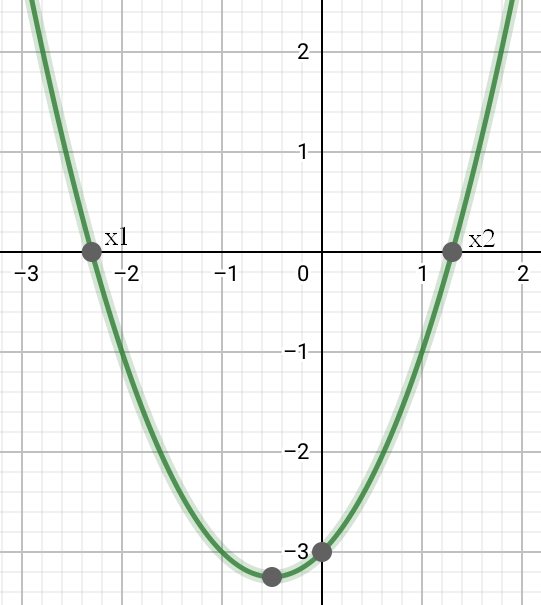
\includegraphics[scale=0.5]{2degre.png}
		\caption{Fonction polynôme de la forme $f(x)=ax^{2}+bx+c$ [GeoGebra]}
	\end{figure}
	
	$$ 0=a(x+\dfrac{b}{2a})^{2}-\dfrac{b^{2}-4ac}{4a} \Leftrightarrow a(x+\dfrac{b}{2a})^{2}=\dfrac{b^{2}-4ac}{4a}$$
	$$\Leftrightarrow (x+\dfrac{b}{2a})^{2}=\dfrac{b^{2}-4ac}{4a^{2}} \Leftrightarrow x+\dfrac{b}{2a}=\pm\dfrac{\sqrt{b^{2}-4ac}}{\sqrt{4a^{2}}}$$
	$$\Leftrightarrow x+\dfrac{b}{2a}=\pm\dfrac{\sqrt{b^{2}-4ac}}{2a}$$
	\begin{center}
		Soit $\boxed{x1=\dfrac{-b-\sqrt{b^{2}-4ac}}{2a}}$ et $\boxed{x2=\dfrac{-b+\sqrt{b^{2}-4ac}}{2a}}$
	\end{center}
\end{document}  % Fin du document